
\subsubsection{Bayesian Inverse Problem}
\label{sec:bayesian}
As discussed in Section \ref{sec:problem:bayesian},
we use the pCN method of \cite{Cotter_2013} to draw samples from the posterior distribution of initial vorticities in the Navier-Stokes equation given sparse, noisy observations at time $T=50$. We compare the Fourier neural operator acting as a surrogate model with the traditional solvers used to generate our train-test data (both run on GPU). We generate 25,000 samples from the posterior (with a 5,000 sample burn-in period), requiring 30,000 evaluations of the forward operator.
%Given a prior, we run \zongyi{number A} MCMC steps and evaluate \zongyi{number B} instances of the forward map with Fourier neural operator and the traditional solver respectively. 

As shown in Figure \ref{fig:baysian}, FNO and the traditional solver recover almost the same posterior mean which, when pushed forward, recovers well the later-time solution of the Navier-Stokes equation.
In sharp contrast, FNO takes $0.005s$ to evaluate a single instance while the traditional solver, after being optimized to use the largest possible internal time-step which does not lead to blow-up, takes $2.2s$. This amounts to $2.5$ minutes for the MCMC using FNO and over $18$ hours for the traditional solver. Even if we account for data generation and training time (offline steps) which take $12$ hours, using FNO is still faster. Once trained, FNO can be used to quickly perform multiple MCMC runs for different initial conditions and observations, while the traditional solver will take $18$ hours for every instance. Furthermore, since FNO is differentiable, it can easily be applied to PDE-constrained optimization problems in which
adjoint calculations are used as part of the solution procedure.

%It is because data-driven methods such as FNO do not require roll-out in time; it has $4$ Fourier layers in total, while the traditional solvers need to have a time step $\Delta t = 0.01$ to maintain a reasonable accuracy. Other reasons could attribute to better parallelization of deep learning methods on GPU. And we acknowledge there could be more efficient implementation of the traditional solvers. The inverse problems of Burgers and Darcy have a similar result \zongyi{a figure in the appendix}. 

\begin{figure}[ht]
    \centering
    \begin{subfigure}[b]{0.32\textwidth}
        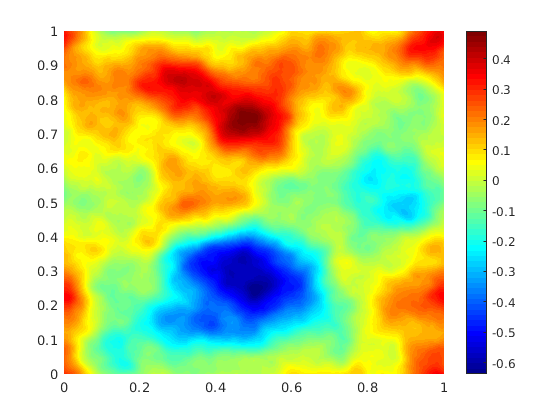
\includegraphics[width=\textwidth]{Figs/u_truth.png}
        %\caption{\(\mug\)}
    \end{subfigure}
    \begin{subfigure}[b]{0.32\textwidth}
        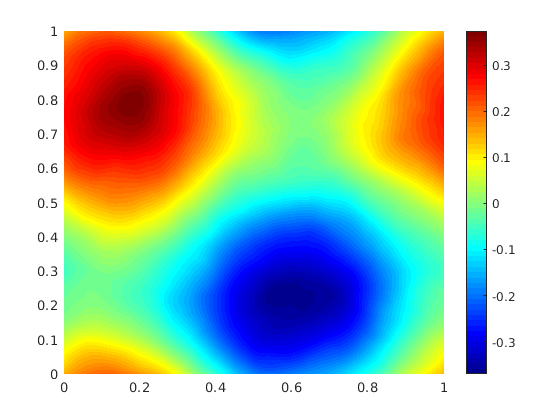
\includegraphics[width=\textwidth]{Figs/umean_truth.png}
        %\caption{\(\mul\)}
    \end{subfigure}
    \begin{subfigure}[b]{0.32\textwidth}
        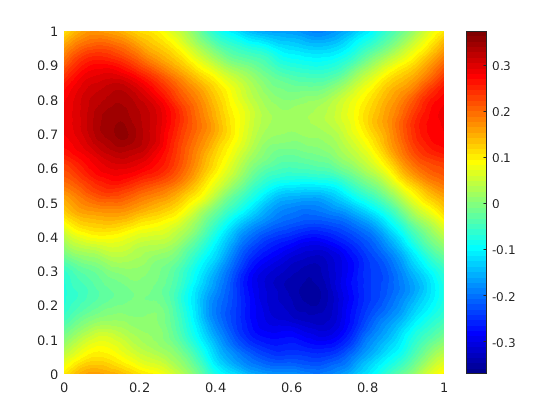
\includegraphics[width=\textwidth]{Figs/umean_approx.png}
        %\caption{\(\mup\)}
    \end{subfigure}
    
    \begin{subfigure}[b]{0.32\textwidth}
        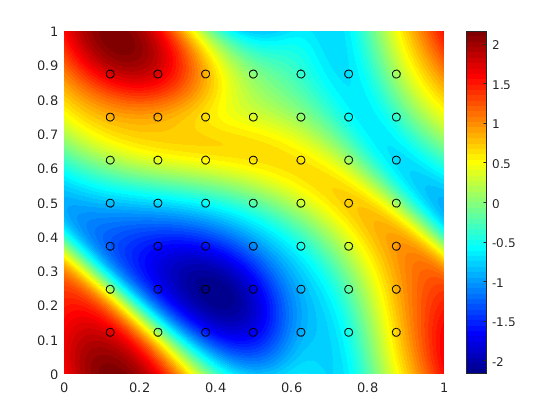
\includegraphics[width=\textwidth]{Figs/gu_truth.png}
        %\caption{\(\mug\)}
    \end{subfigure}
    \begin{subfigure}[b]{0.32\textwidth}
        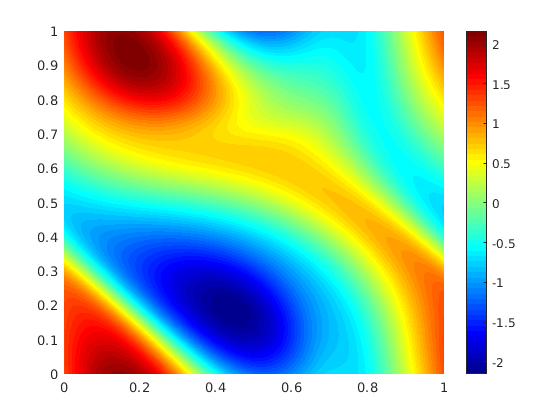
\includegraphics[width=\textwidth]{Figs/gumean_truth.png}
        %\caption{\(\mul\)}
    \end{subfigure}
    \begin{subfigure}[b]{0.32\textwidth}
        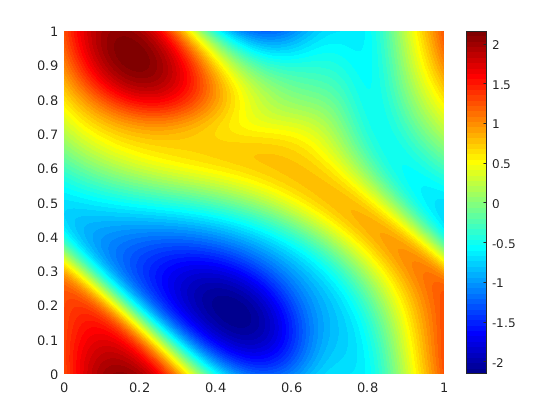
\includegraphics[width=\textwidth]{Figs/gumean_approx.png}
        %\caption{\(\mup\)}
    \end{subfigure}
        \caption{Results of the Bayesian inverse problem for the Navier-Stokes equation. } 
    \label{fig:baysian} 
\small{ The top left panel shows the true initial vorticity while bottom left panel shows the true observed vorticity at $T=50$ with black dots indicating the locations of the observation points placed on a $7 \times 7$ grid. The top middle panel shows the posterior mean of the initial vorticity given the noisy observations estimated with MCMC using the traditional solver, while the top right panel shows the same thing but using FNO as a surrogate model. The bottom middle and right panels show the vorticity at $T=50$ when the respective approximate posterior means are used as initial conditions. }
\end{figure}